\documentclass{article}
\usepackage[utf8]{inputenc}
\usepackage{hyperref}
\usepackage{graphicx}



\title{Project report}
\author{Maximilián Zivák}
\date{June 2022}

\begin{document}

\maketitle

\section{Introduction}
The goal of this project is to parse and visualize data provided by IMDB, with heavy focus on different directors of movies/TV Shows, using flask and SQLite3.
\section{Methods}
IMDB provides tsv files with data on many movies and crews(writers, directors), these tsv files can be downloaded and injected into an SQL database with python. This approach seems the most reasonable since official IMDB API is only available on request and open source APIs are very limited in their request. So we can use the injected tsv data for the most part and use our limited API calls sparingly.
\newline
For visualization, JS library \href{https://developers.google.com/chart/interactive/docs/}{Google charts} is sufficient. So we can present our data as a website running on a flask server. Flask supports jinja2 templating language so sending data into an HTML file is fairly trivial, without needless use of jqueries or such.
\section{Results}
Result is an interactive web page which allows us to look at top 10 movies of a director, their favourite actors and ratings of their movies.
\newline
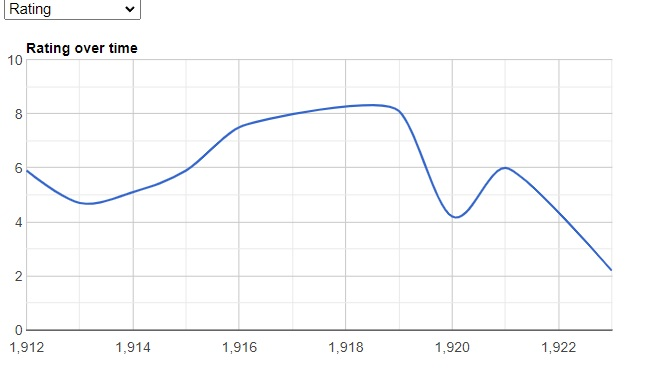
\includegraphics[Chart of average ratings over time]{chart}
\section{Discussion}
I ran into some major problems while trying to create a DB out of tsv files (ran out of disk space), had to bandaid fix it using maxEntries variable. Also I'm inexperienced when it comes to CSS/HTML/JS and frontend isn't my strongest suite so the site looks terrible. On the other hand I've learned a lot about wonders of weakly typed languages and jinja2.
\end{document}
